\documentclass[]{article}
\usepackage{pgfplots}
\usepackage{tikz}
\usepackage{graphicx}
\usetikzlibrary{positioning,arrows.meta}
\tikzset{>=Latex}

%cbbcolors
\colorlet{cbbinit}{green}
\definecolor{cbbmed}{rgb}{1,1,-1}
\definecolor{cbbext}{rgb}{-0.5,-0.5,1}
%glycolors
\colorlet{glyinit}{magenta}
\definecolor{glymed}{rgb}{-0.5,-0.5,1}
\definecolor{glyext}{rgb}{1,-0.5,-0.5}
\colorlet{glyinter}{glymed!50!glyext}
%ptscolors
\colorlet{ptsinit}{cyan}
\definecolor{ptsmed}{rgb}{-0.5,-0.5,1}
\colorlet{ptsext}{green}
\colorlet{gluccol}{green!50!black}
\def\highlightrad{0.2cm}
%glucose data
\colorlet{branchout}{red}
\colorlet{autocatacyc}{blue}
\colorlet{autocataby}{cyan!50}
\def\glucmaxflux{0.2mm}
\def\glucpgi{5.7*\glucmaxflux}
\def\gluccappgi{\glucpgi}
\def\glucpfk{7.06*\glucmaxflux}
\def\glucfba{7.06*\glucmaxflux}
\def\gluctpi{7.06/2*\glucmaxflux}
\def\glucgap{15.71/2*\glucmaxflux}
\def\glucpgk{15.71/2*\glucmaxflux}
\def\glucgpm{14.56/2*\glucmaxflux}
\def\gluceno{14.56/2*\glucmaxflux}
\def\glucpyk{2.49/2*\glucmaxflux}
\def\gluccappyk{\glucpyk/0.33}
\def\glucppc{2.45/2*\glucmaxflux}
\def\gluccapppc{\glucppc/0.47}
\def\gluczwf{3.92*\glucmaxflux}
\def\gluccapzwf{\gluczwf/0.547}
\def\glucpts{9.65*\glucmaxflux}
\def\gluccappts{\glucpts}
%\def\glucrpi{1.43*\glucmaxflux}
%\def\gluccaprpi{\glucrpi/0.47}
%\def\glucrpe{1.4*\glucmaxflux}
%\def\gluccaprpe{\glucrpe/0.26}
%\def\glucgnd{2.83*\glucmaxflux}
%\def\gluccapgnd{\glucgnd/0.32}
%\def\glucedd{1.09*\glucmaxflux}
%\def\gluccapedd{\glucedd/0.58}
%fructose data
\def\frucmaxflux{0.2mm}
%\def\frucpgi{5.7*\frucmaxflux} needs update and descision if relevant
%\def\fruccappgi{\frucpgi}
\def\frucfbp{2.46*\frucmaxflux}
\def\fruccapfbp{\frucfbp}
\def\frucfba{5.87*\frucmaxflux}
\def\fruccapfba{\frucfba/0.71}
\def\fructpi{5.87/2*\frucmaxflux}
\def\frucgap{13.46/2*\frucmaxflux}
\def\frucpgk{13.46/2*\frucmaxflux}
\def\frucgpm{12.6/2*\frucmaxflux}
\def\fruceno{12.6/2*\frucmaxflux}
\def\frucpyk{0.67/2*\frucmaxflux}
\def\fruccappyk{\frucpyk/0.064}
\def\frucppc{3.55/2*\frucmaxflux}
\def\fruccapppc{\frucppc/0.5}
%\def\fruczwf{3.92*\frucmaxflux}
%\def\fruccapzwf{\fruczwf/0.547}
\def\frucpts{8.33*\frucmaxflux}
\def\fruccappts{\frucpts}

%Galactose data
\def\galmaxflux{0.5mm}
\def\galglt{1.52*\galmaxflux}
\def\galcapglt{\galglt/0.21}
\def\galacn{1.52*\galmaxflux*1.5}
\def\galacea{1.02*\galmaxflux}
\def\galcapacea{\galacea/0.29}
\def\galaceb{1.02*\galmaxflux}
\def\galsdh{1.26*\galmaxflux}
\def\galfum{1.26*\galmaxflux}
\def\galmdh{2.28*\galmaxflux}
\def\galpck{0.85*\galmaxflux}
\def\galcappck{\galpck/0.26}
\def\galicd{0.5*\galmaxflux}
\def\galcapicd{\galicd/0.09}
%\def\galx{0.29*\galmaxflux}%% name reaction and find capacity
%acetate data
\def\acemaxflux{0.2mm}
\def\aceglt{8.83*\acemaxflux}
\def\acecapglt{\aceglt/0.68}
\def\aceacn{8.83*\acemaxflux*1.5}
\def\aceacea{4.14*\acemaxflux}
\def\acecapacea{\aceacea}
\def\aceaceb{4.14*\acemaxflux}
\def\acesdh{8.4*\acemaxflux}
\def\acefum{8.4*\acemaxflux}
\def\acemdh{10.67*\acemaxflux}
%\def\acex{0.5*\acemaxflux}
\def\acemae{1.87*\acemaxflux}
\def\acecapmae{\acemae/0.13}
\def\acepck{3.11*\acemaxflux}
\def\acecappck{\acepck/0.75}
\def\aceicd{4.7*\acemaxflux}
\def\acecapicd{\aceicd/0.63}
%mal=oaa=4c
%cit=icit=6c
%gly=2cj
\begin{document}

\begin{figure}
    \resizebox{1\linewidth}{!}{
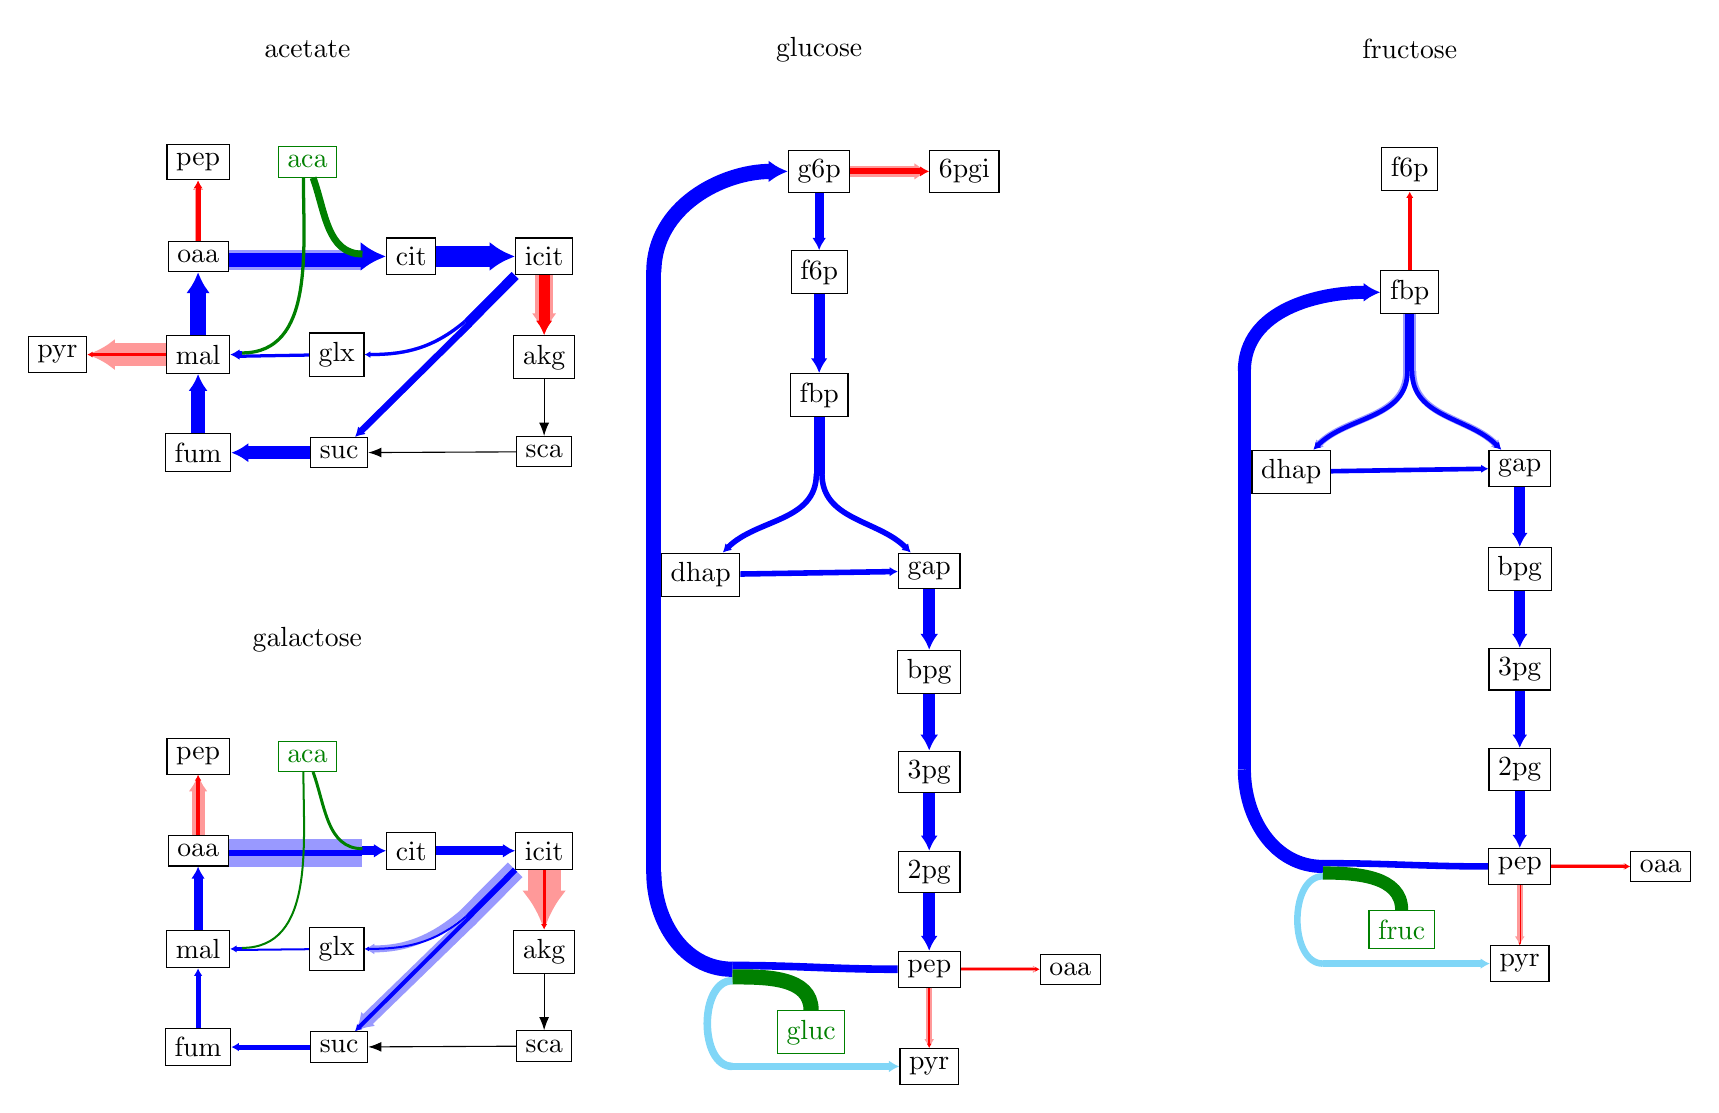
\begin{tikzpicture}
  \begin{scope}[shift={(-6cm,-7.5cm)}]
    \node[] (galactose) {galactose};
    \node[rectangle,draw,gluccol,below=of galactose] (aca) {aca};
    \node[shape=coordinate,below=of aca] (dummyglta) {};
    \node[rectangle,draw,left=of dummyglta] (oaa) {oaa};
    \node[rectangle,draw] at (aca -| oaa) (pep) {pep};
    \node[rectangle,draw,right=of dummyglta] (cit) {cit};
    \node[rectangle,draw,right=of cit] (icit) {icit};
    \node[rectangle,draw,below=of icit.center] (akg) {akg};
    \node[rectangle,draw,below=of akg.center] (sca) {sca};
    \node[rectangle,draw,below=of oaa.center] (mal) {mal};
    \node[rectangle,draw,below=of mal.center] (fum) {fum};
    \node[rectangle,draw,right=of mal] (glx) {glx};
    \node[rectangle,draw,right=of fum] (suc) {suc};
    \path[] (oaa) -- (cit) node [pos=0.85,shape=coordinate] (midglta) {};
    \draw[line width=\galcapglt,autocatacyc!40] ([yshift=-0.35*\galglt]oaa.east) -- ([yshift=-0.35*\galglt]midglta);
    \draw[line width=\galglt,autocatacyc] ([yshift=-0.35*\galglt]oaa.east) -- ([yshift=-0.35*\galglt]midglta);
    \draw[-{Latex[scale=0.25,angle'=60]},line width=\galglt*1.5,autocatacyc] (midglta) -- (cit);
    \draw[-{Latex[scale=0.25,angle'=60]},line width=\galcappck,branchout!40] (oaa) -- (pep);
    \draw[-{Latex[scale=0.25,angle'=60]},line width=\galpck,branchout] (oaa) -- (pep);
    \draw [gluccol,line width=0.5*\galglt] (aca) [out=-70,in=180] to ([yshift=0.35*\galglt]midglta);
    \draw[-{Latex[scale=0.25,angle'=60]},line width=\galacn,autocatacyc] (cit) -- (icit);
    \path[] (icit.south west) -- (suc) node [pos=0.3,shape=coordinate] (midacea) {};
    \draw[line width=\galcapacea*1.5,autocatacyc!40] (icit.south west) -- (midacea);
    \draw[-{Latex[scale=0.25,angle'=60]},line width=\galcapacea,autocatacyc!40] ([xshift=\galcapacea*0.35]midacea) -- ([xshift=\galcapacea*0.4]suc);
    \draw[-{Latex[scale=0.25,angle'=60]},line width=\galcapacea*0.5,autocatacyc!40] ([shift={(-\galcapacea*0.35,\galcapacea*0.35)}]midacea) [out=220,in=0] to (glx);
    \draw[line width=\galacea*1.5,autocatacyc] (icit.south west) -- (midacea);
    \draw[-{Latex[scale=0.25,angle'=60]},line width=\galacea,autocatacyc] ([xshift=\galacea*0.4]midacea) -- ([xshift=\galacea*0.4]suc);
    \draw[-{Latex[scale=0.25,angle'=60]},line width=\galacea*0.5,autocatacyc] ([shift={(-\galacea*0.35,\galacea*0.35)}]midacea) [out=220,in=0] to (glx);
    \draw[-{Latex[scale=0.25,angle'=60]},line width=\galcapicd*1.5,branchout!40] (icit) -- (akg);
    \draw[-{Latex[scale=0.25,angle'=60]},line width=\galicd*1.5,branchout] (icit) -- (akg);
    \draw[->] (akg) -- (sca);
    \draw[->] (sca) -- (suc);
    \draw[-{Latex[scale=0.25,angle'=60]},line width=\galsdh,autocatacyc] (suc) -- (fum);
    \draw[-{Latex[scale=0.25,angle'=60]},line width=\galfum,autocatacyc](fum) -- (mal);
    \path[] (glx) -- (mal) node [pos=0.85,shape=coordinate] (midaceb) {};
    \draw[line width=\galaceb*0.5,autocatacyc] ([yshift=-0.25*\galaceb]glx) -- ([yshift=-0.25*\galaceb]midaceb);
    \draw[gluccol,line width=0.5*\galaceb] ([xshift=-0.5mm]aca.south) [out=-90,in=0] to ([yshift=0.25*\galaceb]midaceb);
    \draw[-{Latex[scale=0.25,angle'=60]},line width=\galaceb,autocatacyc] (midaceb) -- (mal);
    \draw[-{Latex[scale=0.25,angle'=60]},line width=\galmdh,autocatacyc] (mal) -- (oaa);
  \end{scope}
  \begin{scope}[shift={(-6cm,0cm)}]
    \node[] (acetate) {acetate};
    \node[rectangle,draw,gluccol,below=of acetate] (aca) {aca};
    \node[shape=coordinate,below=of aca] (dummyglta) {};
    \node[rectangle,draw,left=of dummyglta] (oaa) {oaa};
    \node[rectangle,draw] at (aca -| oaa) (pep) {pep};
    \node[rectangle,draw,right=of dummyglta] (cit) {cit};
    \node[rectangle,draw,right=of cit] (icit) {icit};
    \node[rectangle,draw,below=of icit.center] (akg) {akg};
    \node[rectangle,draw,below=of akg.center] (sca) {sca};
    \node[rectangle,draw,below=of oaa.center] (mal) {mal};
    \node[rectangle,draw,below=of mal.center] (fum) {fum};
    \node[rectangle,draw,right=of mal] (glx) {glx};
    \node[rectangle,draw,left=of mal] (pyr) {pyr};
    \node[rectangle,draw,right=of fum] (suc) {suc};
    \path[] (oaa) -- (cit) node [pos=0.85,shape=coordinate] (midglta) {};
    \draw[line width=\acecapglt,autocatacyc!40] ([yshift=-0.25*\aceglt]oaa.east) -- ([yshift=-0.25*\aceglt]midglta);
    \draw[line width=\aceglt,autocatacyc] ([yshift=-0.25*\aceglt]oaa.east) -- ([yshift=-0.25*\aceglt]midglta);
    \draw[-{Latex[scale=0.25,angle'=60]},line width=\aceglt*1.5,autocatacyc] (midglta) -- (cit);
    \draw[-{Latex[scale=0.25,angle'=60]},line width=\acecappck,branchout!40] (oaa) -- (pep);
    \draw[-{Latex[scale=0.25,angle'=60]},line width=\acepck,branchout] (oaa) -- (pep);
    \draw[-{Latex[scale=0.25,angle'=60]},line width=\acecapmae,branchout!40] (mal) -- (pyr);
    \draw[-{Latex[scale=0.25,angle'=60]},line width=\acemae,branchout] (mal) -- (pyr);
    \draw [gluccol,line width=0.5*\aceglt] (aca) [out=-70,in=180] to ([yshift=0.4*\galglt]midglta);
    \draw[-{Latex[scale=0.25,angle'=60]},line width=\aceacn,autocatacyc] (cit) -- (icit);
    \path[] (icit.south west) -- (suc) node [pos=0.3,shape=coordinate] (midacea) {};
    \draw[line width=\acecapacea*1.5,autocatacyc!40] (icit.south west) -- (midacea);
    \draw[-{Latex[scale=0.25,angle'=60]},line width=\acecapacea,autocatacyc!40] ([xshift=\acecapacea*0.35]midacea) -- ([xshift=\acecapacea*0.4]suc);
    \draw[-{Latex[scale=0.25,angle'=60]},line width=\acecapacea*0.5,autocatacyc!40] ([shift={(-\acecapacea*0.35,\acecapacea*0.35)}]midacea) [out=220,in=0] to (glx);
    \draw[line width=\aceacea*1.5,autocatacyc] (icit.south west) -- (midacea);
    \draw[-{Latex[scale=0.25,angle'=60]},line width=\aceacea,autocatacyc] ([xshift=\aceacea*0.4]midacea) -- ([xshift=\aceacea*0.4]suc);
    \draw[-{Latex[scale=0.25,angle'=60]},line width=\aceacea*0.5,autocatacyc] ([shift={(-\aceacea*0.35,\aceacea*0.35)}]midacea) [out=220,in=0] to (glx);
    \draw[-{Latex[scale=0.25,angle'=60]},line width=\acecapicd*1.5,branchout!40] (icit) -- (akg);
    \draw[-{Latex[scale=0.25,angle'=60]},line width=\aceicd*1.5,branchout] (icit) -- (akg);
    \draw[->] (akg) -- (sca);
    \draw[->] (sca) -- (suc);
    \draw[-{Latex[scale=0.25,angle'=60]},line width=\acesdh,autocatacyc] (suc) -- (fum);
    \draw[-{Latex[scale=0.25,angle'=60]},line width=\acefum,autocatacyc](fum) -- (mal);
    \path[] (glx) -- (mal) node [pos=0.85,shape=coordinate] (midaceb) {};
    \draw[line width=\aceaceb*0.5,autocatacyc] ([yshift=-0.25*\aceaceb]glx) -- ([yshift=-0.25*\aceaceb]midaceb);
    \draw[gluccol,line width=0.5*\aceaceb] ([xshift=-0.5mm]aca.south) [out=-90,in=0] to ([yshift=0.25*\aceaceb]midaceb);
    \draw[-{Latex[scale=0.25,angle'=60]},line width=\aceaceb,autocatacyc] (midaceb) -- (mal);
    \draw[-{Latex[scale=0.25,angle'=60]},line width=\acemdh,autocatacyc] (mal) -- (oaa);
 
  \end{scope}
  %glucose
  \begin{scope}[shift={(0.5cm,0cm)}]
    \node[] (glucose) {glucose};
    \node[rectangle,draw,below= of glucose] (g6p) {g6p};
    \node[rectangle,draw,below=of g6p.center] (f6p) {f6p};
    \node[rectangle,draw,below=of f6p] (fbp) {fbp};
    \node[rectangle,draw,shape=coordinate,below=of fbp.center](fbamid) {};
    \node[rectangle,draw,below left=of fbamid.center] (dhap) {dhap};
    \node[rectangle,draw,below right=of fbamid] (gap) {gap};
    \node[rectangle,draw,below=of gap.center] (bpg) {bpg};
    \node[rectangle,draw,below=of bpg.center] (3pg) {3pg};
    \node[rectangle,draw,below=of 3pg.center] (2pg) {2pg};
    \node[rectangle,draw,below=of 2pg.center] (pep) {pep};
    \node[rectangle,draw,right=of pep] (oaa) {oaa};
    \node[rectangle,draw,below=of pep.center] (pyr) {pyr};
    \node[rectangle,draw,right=of g6p] (6pgi) {6pgi};
    \draw[-{Latex[scale=0.25,angle'=60]},line width=\glucpgi,autocatacyc] (g6p) -- (f6p);
    \draw[-{Latex[scale=0.25,angle'=60]},line width=\glucpfk,autocatacyc] (f6p.south) -- (fbp.north);
    \draw [line width=\glucfba,autocatacyc] (fbp) [out=-90,in=90] to (fbamid);
    \draw [-{Latex[scale=0.25,angle'=60]},line width=\glucfba/2,autocatacyc] ([xshift=-\glucfba/4]fbamid) [out=-90,in=45] to (dhap);
    \draw [-{Latex[scale=0.25,angle'=60]},line width=\glucfba/2,autocatacyc] ([xshift=\glucfba/4]fbamid) [out=-90,in=135] to (gap);
    \draw [-{Latex[scale=0.25,angle'=60]},line width=\gluctpi,autocatacyc] (dhap) -- (gap);

    \draw[-{Latex[scale=0.25,angle'=60]},line width=\glucgap,autocatacyc] (gap) -- (bpg);
    \draw[-{Latex[scale=0.25,angle'=60]},line width=\glucpgk,autocatacyc] (bpg) -- (3pg);
    \draw[-{Latex[scale=0.25,angle'=60]},line width=\glucgpm,autocatacyc] (3pg) -- (2pg);
    \draw[-{Latex[scale=0.25,angle'=60]},line width=\gluceno,autocatacyc] (2pg) -- (pep);
    \draw[-{Latex[scale=0.25,angle'=60]},line width=\gluccappyk,branchout!40] (pep) -- (pyr);
    \draw[-{Latex[scale=0.25,angle'=60]},line width=\glucpyk,branchout] (pep) -- (pyr);
    \draw[-{Latex[scale=0.25,angle'=60]},line width=\gluccapppc,branchout!40] (pep) -- (oaa);
    \draw[-{Latex[scale=0.25,angle'=60]},line width=\glucppc,branchout] (pep) -- (oaa);
    \draw[-{Latex[scale=0.25,angle'=60]},line width=\gluccapzwf,branchout!40] (g6p) -- (6pgi);
    \draw[-{Latex[scale=0.25,angle'=60]},line width=\gluczwf,branchout] (g6p) -- (6pgi);
    \node[rectangle,draw,shape=coordinate,left=of dhap.center] (pts2) {};
    \node[rectangle,draw,gluccol,shift={(-1.5,-0.8)}] at (pep.center) (gluc) {gluc};
    \node[rectangle,draw,shape=coordinate,left=2.5cm of pep.center] (pts3) {};
    \draw[line width=\glucpts/2,autocatacyc] ([yshift=\glucpts/4]pep) [out=180,in=0] to ([yshift=\glucpts/4]pts3);
    \draw[gluccol,line width=\glucpts] ([yshift=-\glucpts/2]gluc) [out=90,in=0] to ([yshift=-\glucpts/2]pts3);
    \node[rectangle,draw,shape=coordinate,left=2.5cm of pyr.center] (pts5) {};
    \draw[line width=\glucpts/2,autocataby] ([yshift=-3*\glucpts/4]pts3) [out=180,in=180] to (pts5);
    \draw[-{Latex[scale=0.25,angle'=60]},line width=\glucpts/2,autocataby] (pts5) [out=0,in=180] to (pyr);
    \node[rectangle,draw,shape=coordinate,left=2.1cm of f6p.center] (ptstop) {};
    \node[rectangle,draw,shape=coordinate] at(ptstop |- 2pg.center) (ptsbottom) {};
    \draw[line width=\glucpts,autocatacyc] (pts3) [in=-90,out=180] to (ptsbottom);
    \draw[line width=\glucpts,autocatacyc] (ptsbottom) [in=-90,out=90] to (ptstop);
    \draw[-{Latex[scale=0.25,angle'=60]},line width=\glucpts,autocatacyc] (ptstop) [in=180,out=90] to (g6p);
  \end{scope}
  %fructose
  \begin{scope}[shift={(8cm,0cm)}]
    \node[] (fructose) {fructose};
    \node[rectangle,draw,below=of fructose] (f6p) {f6p};
    \node[rectangle,draw,below=of f6p] (fbp) {fbp};
    \node[rectangle,draw,shape=coordinate,below=of fbp.center](fbamid) {};
    \node[rectangle,draw,below left=of fbamid.center] (dhap) {dhap};
    \node[rectangle,draw,below right=of fbamid] (gap) {gap};
    \node[rectangle,draw,below=of gap.center] (bpg) {bpg};
    \node[rectangle,draw,below=of bpg.center] (3pg) {3pg};
    \node[rectangle,draw,below=of 3pg.center] (2pg) {2pg};
    \node[rectangle,draw,below=of 2pg.center] (pep) {pep};
    \node[rectangle,draw,right=of pep] (oaa) {oaa};
    \node[rectangle,draw,below=of pep.center] (pyr) {pyr};
    \draw[-{Latex[scale=0.25,angle'=60]},line width=\frucfbp,branchout] (fbp.north)-- (f6p.south) ;
    \draw [line width=\fruccapfba,autocatacyc!40] (fbp) [out=-90,in=90] to (fbamid);
    \draw [-{Latex[scale=0.25,angle'=60]},line width=\fruccapfba/2,autocatacyc!40] ([xshift=-\fruccapfba/4]fbamid) [out=-90,in=45] to (dhap);
    \draw [-{Latex[scale=0.25,angle'=60]},line width=\fruccapfba/2,autocatacyc!40] ([xshift=\fruccapfba/4]fbamid) [out=-90,in=135] to (gap);
    \draw [line width=\frucfba,autocatacyc] (fbp) [out=-90,in=90] to (fbamid);
    \draw [-{Latex[scale=0.25,angle'=60]},line width=\frucfba/2,autocatacyc] ([xshift=-\frucfba/4]fbamid) [out=-90,in=45] to (dhap);
    \draw [-{Latex[scale=0.25,angle'=60]},line width=\frucfba/2,autocatacyc] ([xshift=\frucfba/4]fbamid) [out=-90,in=135] to (gap);
    \draw [-{Latex[scale=0.25,angle'=60]},line width=\fructpi,autocatacyc] (dhap) -- (gap);

    \draw[-{Latex[scale=0.25,angle'=60]},line width=\frucgap,autocatacyc] (gap) -- (bpg);
    \draw[-{Latex[scale=0.25,angle'=60]},line width=\frucpgk,autocatacyc] (bpg) -- (3pg);
    \draw[-{Latex[scale=0.25,angle'=60]},line width=\frucgpm,autocatacyc] (3pg) -- (2pg);
    \draw[-{Latex[scale=0.25,angle'=60]},line width=\fruceno,autocatacyc] (2pg) -- (pep);
    \draw[-{Latex[scale=0.25,angle'=60]},line width=\gluccappyk,branchout!40] (pep) -- (pyr);
    \draw[-{Latex[scale=0.25,angle'=60]},line width=\frucpyk,branchout] (pep) -- (pyr);
    \draw[-{Latex[scale=0.25,angle'=60]},line width=\gluccapppc,branchout!40] (pep) -- (oaa);
    \draw[-{Latex[scale=0.25,angle'=60]},line width=\frucppc,branchout] (pep) -- (oaa);
    \node[rectangle,draw,shape=coordinate,left=of dhap.center] (pts2) {};
    \node[rectangle,draw,shape=coordinate,left=2.5cm of pep.center] (pts3) {};
    \draw[line width=\frucpts/2,autocatacyc] ([yshift=\frucpts/4]pep) [out=180,in=0] to ([yshift=\frucpts/4]pts3);
    \node[rectangle,draw,shape=coordinate,left=2.5cm of pyr.center] (pts5) {};
    \draw[line width=\frucpts/2,autocataby] ([yshift=-3*\frucpts/4]pts3) [out=180,in=180] to (pts5);
    \draw[-{Latex[scale=0.25,angle'=60]},line width=\frucpts/2,autocataby] (pts5) [out=0,in=180] to (pyr);
    \node[rectangle,draw,shape=coordinate,left=2.1cm of fbamid] (ptstop) {};
    \node[rectangle,draw,shape=coordinate] at(ptstop |- 2pg.center) (ptsbottom) {};
    \draw[] (pts3) [in=-90,out=180] to (ptsbottom);
    \draw[] (ptsbottom) [in=-90,out=90] to (ptstop);
    \node[rectangle,draw,gluccol,shift={(-1.5,-0.8)}] at (pep.center) (fruc) {fruc};
    \draw[gluccol,line width=\frucpts] ([yshift=-\frucpts/2]fruc) [out=90,in=0] to ([yshift=-\frucpts/2]pts3);
    \draw[line width=\frucpts,autocatacyc] (pts3) [in=-90,out=180] to (ptsbottom);
    \draw[line width=\frucpts,autocatacyc] (ptsbottom) [in=-90,out=90] to (ptstop);
    \draw[-{Latex[scale=0.25,angle'=60]},line width=\frucpts,autocatacyc] (ptstop) [in=180,out=90] to (fbp);
  \end{scope}
  \end{tikzpicture}
}
\caption{
  Major branch points and relative enzyme saturation in operating autocatalytic cycles.
}
\end{figure}
\end{document}
